\subsection{Reconstruction and Identification}
\label{sec:muReco}
\par Every track reconstructed in the Muon Spectrometer is considered a muon track, 
after all ambiguities are resolved. Each of these tracks is further categorized into 
classes upon demanding further identification requirements. Muons identified 
just by tracks from the Muon Spectrometer are classified as {\it Stand-Alone 
Muons (SA)}. As mentioed in Section~\ref{sec:tracking} these tracks are extrapolated to the IP, 
and energy losses from minimal ionizations in the calorimeters are corrected for. 
Muons constructed by combining and matching tracks from the MS and the ID are 
known as {\it Combined (CB)} muons. The overall quality of CB muons is characterized by the significance of 
the ratio of the track charge to its momentum $q/p$, the $\chi^2$ of the combined 
MS-ID fit, and the number of ID track hits. For an ID track to be considered as 
a candidate for matching with an MS track it is required to have at least 1 hit 
in the Pixel Detector, 5 SCT hits, and fewer than 3 Pixel Detector or SCT holes. 
Other types of muons that are rarely used are {\it Segment Tagged (ST)} and 
{\it Calorimeter Tagged (CT)} muons. An ST muon is reconstructed if at least one 
of the MS segments is matched to an ID track, while a CT muon is reconstructed if 
some energy deposits consistent with a muon path in the calorimeters are matched 
to a track in the ID. Purity in these muon classes is ranked as follows: CB, ST, 
SA and CT. Overlaps between classes are resolved in the same order 
of preferrence. CB muons were used in both analyses discussed in this Thesis while 
SA muons are normally used to determine the efficiency of measuring muons with the 
ID. 

\par CB muons used in Run I were required to have at least 3 MDT hits in at least two 
layers. This rule was relaxed to at least 1 MDT layer  and no more than 1 MDT hole in 
the region of $|\eta|<0.1$, which is partially equipped because of service cables.
During Run II muon classes were modified to mimic electron identification classes, 
i.e Loose, Medium and Tight. These classes contain more than one of the CB, ST, SA and 
CT categories. For example, the Medium class is a combination of CB and SA muons. 
For $|\eta|<2.5$ CB muons are used with the same requirements demanded during Run I. For 
$|\eta|>2.5$, which does not have ID tracking, SA muons are used. They are required to have 
hits in at least 3 MDT or CSC layers, and the significance of their $q/p$ is required to be 
less than 7 to reduce contamination from muons from \kaon and  
and \pipm\ decays. Medium muons are used in this Thesis for Run 2 data and CB muons 
are used for Run 1 data.   

\subsection{Measurement of efficiencies, corrections and uncertainties}
\par Just like electron reconstruction, muons reconstruction suffers from inefficiencies 
and energy skews, especially in Monte Carlo simulation. Identification efficiencies in Monte Carlo 
are also not expected to match with those in data.  
Techniques to correct for this are discussed here. 

\subsubsection{Identification Efficiency}
\par Identification and reconstruction 
efficiencies for muons are terms used rather inter-changeably. This 
is because as mentioned before, any track reconstructed in the MS and 
matched to a track in the ID is considered a muon. So, the only efficiency described 
in this text for muons is the identification efficiency, $\epsilon_{id}$. 
Only $\epsilon_{id}$ for muons with $|\eta|<2.5$ is discussed here. Otherwise, the reader 
is encouraged to read Ref~\cite{Aad:2014rra}. For a thorough discussion of muon 
isolation efficiencies the reader is also encouraged to read the same reference.  

\par Since muons with $|\eta|<2.5$ are measured from 
both the ID and MS tracks, the tag-and-probe method is naturally appealing. Given two muons, 
one is used as the tag object and the other as the probe object. The identification efficiency 
can be factorized as  

\begin{equation}
\epsilon_{id} = \epsilon_{id|ID}\times\epsilon_{ID}.
\end{equation}

where $\epsilon_{id|ID}$ is the efficiency of a muon track in the ID to be identified as a muon\footnote{During Run I 
these categories were just CB, ST, CT, etc. During Run II the standard loose, medium, tight working points were 
used.}, and $\epsilon_{ID}$ is the efficiency of a muon track to be reconstructed in the ID. The latter is efficiency 
is difficult to calculate, so it is approximated by $\epsilon_{ID|MS}$, which is the efficiency of 
reconstructing a muon track in the ID given that it has been reconstructed in the MS.  
Ultimately, the efficiencies in data, $\epsilon_{id}^{data}$, and MC, $\epsilon_{id}^{MC}$, are compared 
by taking their ratio as a scale factor. This cancels out any biases stemming from the tag-and-probe 
method.  

\par To cover a wide range of muon $\pt$, efficiency measurements were performed using both 
\Jmm\ and \Zmm\ events from data and MC. 
For \Zmm\ events the tag muon was required to satisfy the following:
\begin{enumerate}
\item medium quality, loose isolation and have $\pT>24~\GeV$; 
\item impact parameter requirements to ensure that it originated from the primary vertex;
\item and be matched to the muon trigger. 
\end{enumerate}
The probe muon was required to have $\pt>10~\GeV$ and be loosely isolated. 
For \Jmm\ the tag muon was required to have $\pT>5~\GeV$, be of medium ID, and be 
matched to the muon trigger. Additionally, for both \Jmm\ and \Zmm the probe muon
was required to have a fully reconstructed muon within $\Delta R< 0.05$ around its location. 

\par Efficiencies were extracted in bins of $\eta,\phi$ and $\pt$, as described in full detail in 
Ref~\cite{Aad:2016jkr}. Figure~\ref{fig:muEff} shows identification efficiencies exctracted from data 
for medium (Run II) and CB (Run I) muons in the region $0.1<|\eta|<2.5$. The high \pt\ region was 
covered by muons from \Zmm\ events while the low \pt\ region was covered by muons 
from \Jmm\ events. Above about 20~\GeV, the efficiency was observed to be independent from 
the muon \pt. Overall, the agreement between data and Monte Carlo simulation was observed 
to be within 1\%.    

\begin{figure}[h]
\begin{subfigure}{0.5\textwidth}
   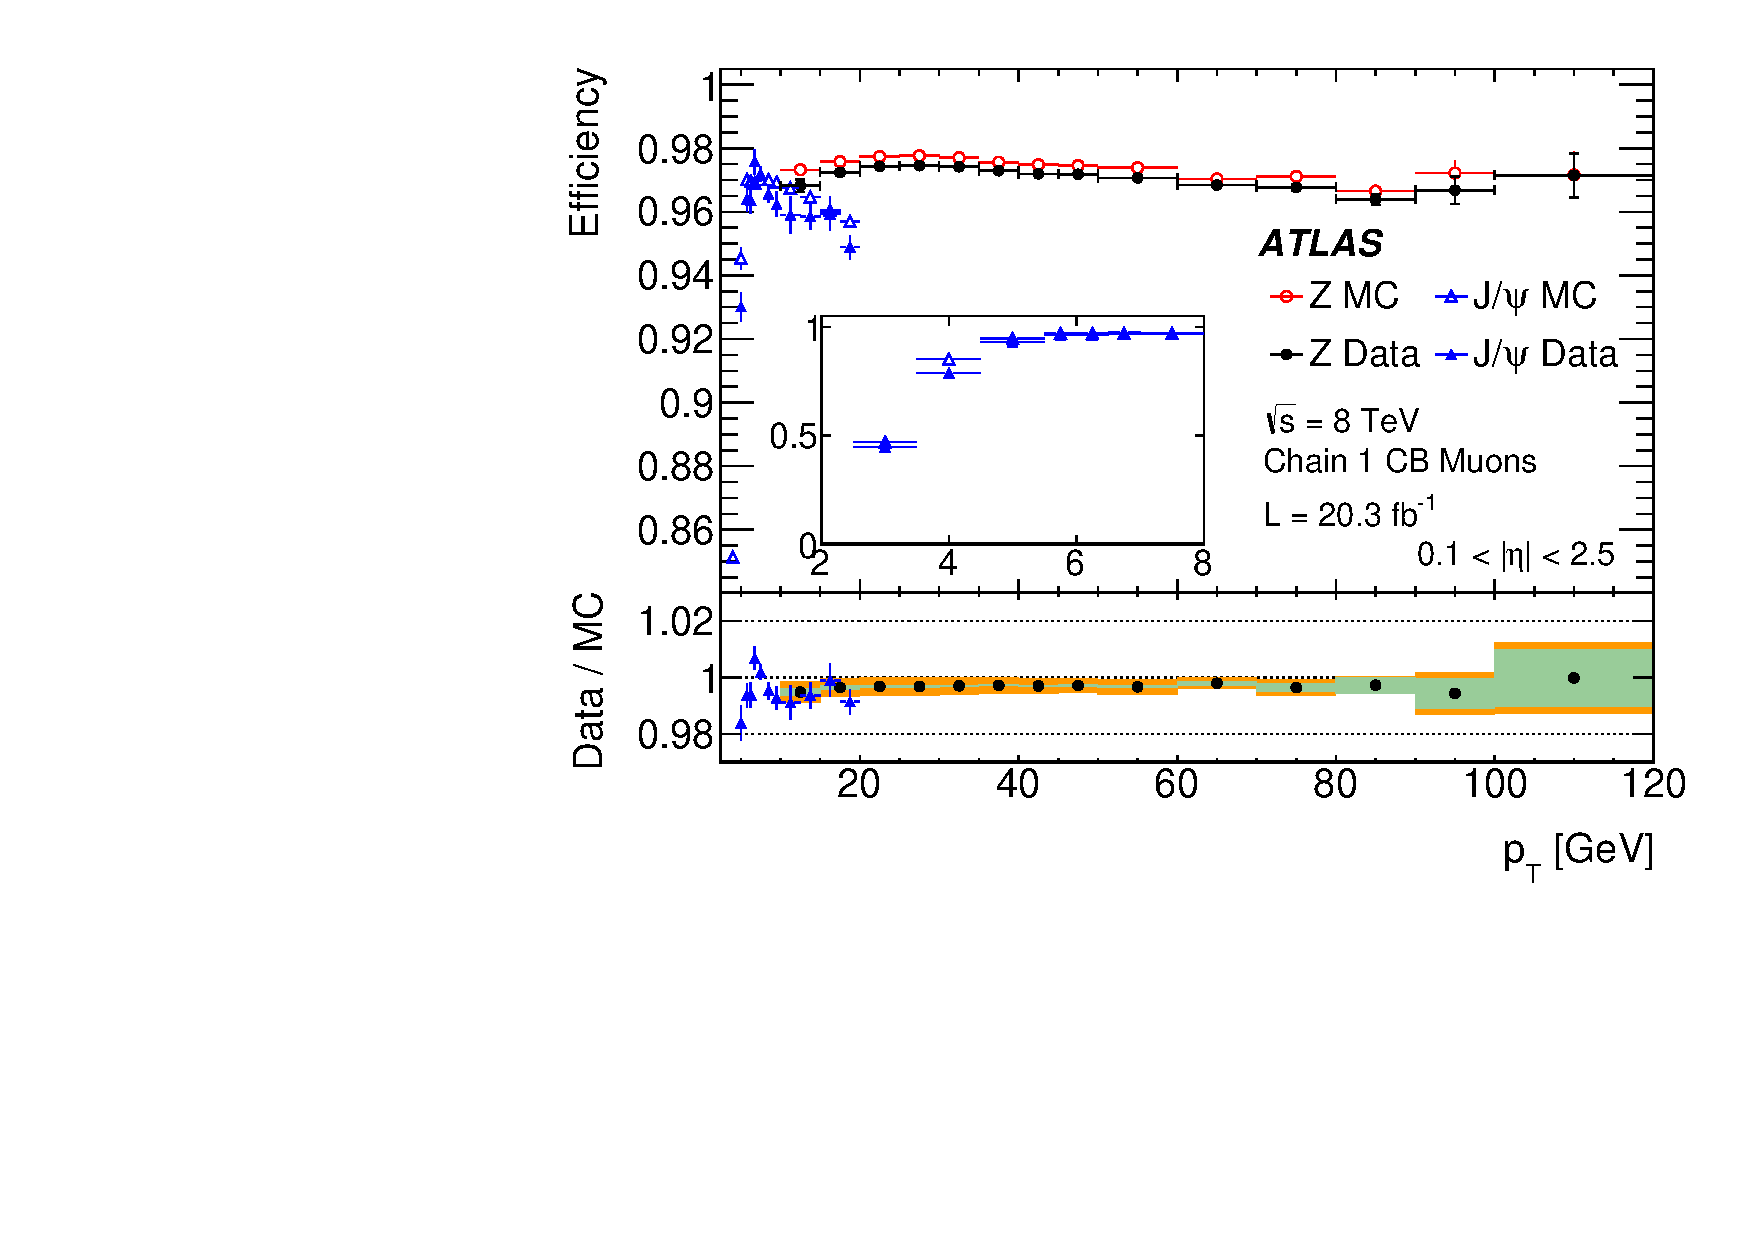
\includegraphics[width=\textwidth]{figures/Full_eff_pt_jpsi_Staco_CB_noCrack.pdf}
	\caption{Run I. Taken from Ref~\cite{Aad:2014rra}}
\end{subfigure} % 
\begin{subfigure}{0.5\textwidth}
   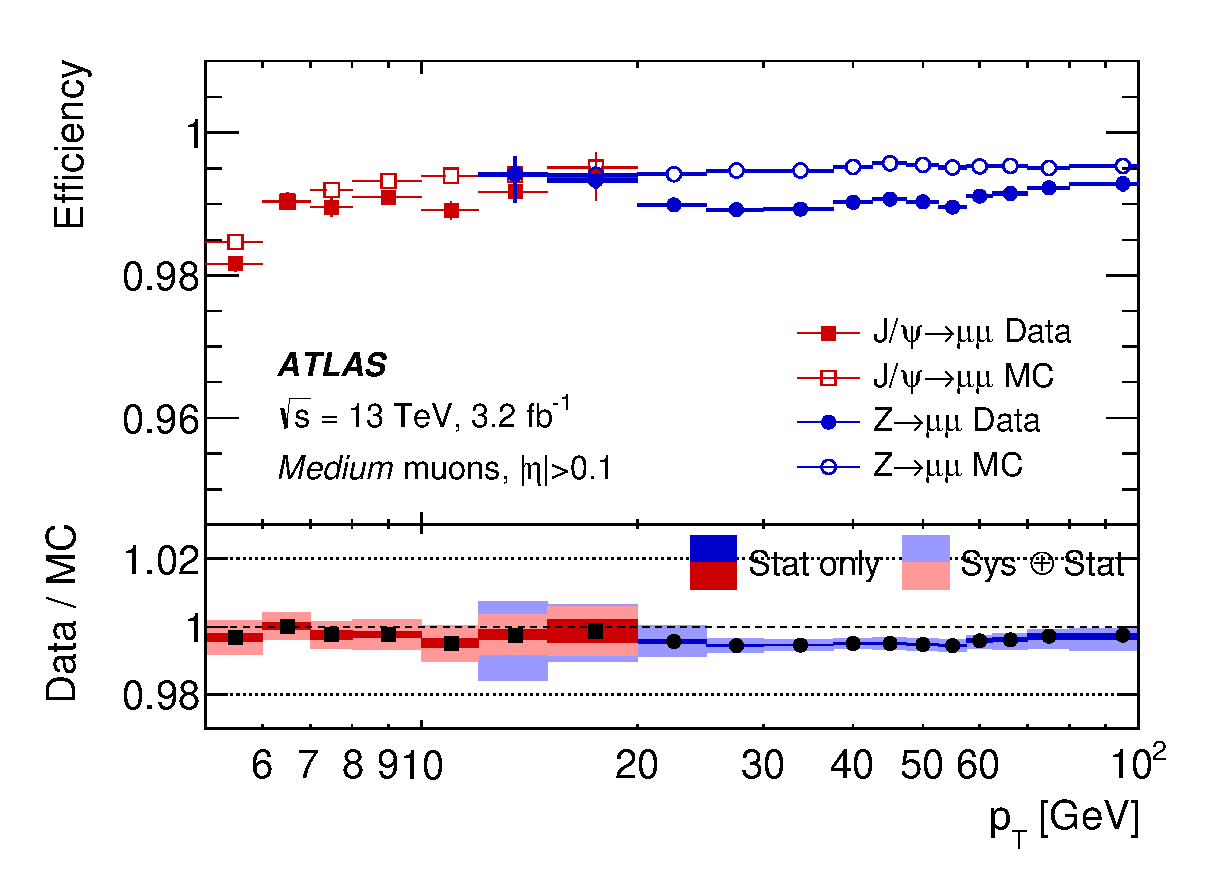
\includegraphics[width=\textwidth]{figures/fig_06.eps}
	\caption{Run II. Taken from Ref~\cite{Aad:2016jkr}}
\end{subfigure}
\caption{Plots of the muon identification efficiencies, binned in \pT. \Zmm\ events were used for high \pt\ muons 
while \Jmm\ events were used for low \pt muons  
}
\label{fig:muEff}
\end{figure}

\par The major systematic uncertainties affecting these results were found to be from the data-driven estimation 
of background processes, choice of cone size used to match probe muons to reconstructed muons, and kinematic 
distribution disagreements between probes in data and Monte Carlo simulation. The uncertainties due to background 
processes was calculated by varying a parameter used in the estimation by $\pm 100\%$. The cone size uncertainties 
were evaluated by varying the cone size by $\pm 50\%$. Distributions of probe kinematics in MC were weighted to 
agree with data. The shift was taken as a systematic uncertainty. After adding these and other~\cite{Aad:2016jkr} 
uncertainties in quadrature, the overall uncertainties on the identification efficiencies were less than 2\%. 
 

\subsubsection{Momentum Scale and Smear} 
\par Just like with electrons, muons may lose energy as they traverse detector material upstream 
of the Muon Spectrometer (MS). This loss may also be mis-modelled in Monte Carlo simulations. 
While losses in the Inner Detector (ID) are very small and taken as negligible, losses the calorimeters 
cannot be neglected. Modelling of the magnetic field integral and detector dimensions in the ID
 and MS in Monte Carlo simulations may also differ from the true physical values. Energy loss and other
forms of mismodelling must therefore be corrected in both data and Monte Carlo simulation. 
Effectively such corrections adjust the muon momentum by scale factors. 

\par Fluctuations in muon energy losses in the calorimeters  
lead to uncertainties in the measured muon momentum. Magnetic field 
inhomogeneities, spatial hits displacements in the ID and MS, and 
misalignment of the MS all lead to larger uncertainties in the measured 
muon \pT\ in both the ID and MS. Accounting for these uncertainties 
broadens (or {\it smears}) the \pT\ resolution in MC to match the data. The corrected muon \pT\ in 
MC can be written as

\begin{equation}
\pT^{corr,MC} = \frac{\pT^{uncorr,MC} + \text{Sum of Scales}}{1 + \text{Sum of Smears}},
\end{equation} 

where the scale and smear corrections are derived from data. 

\par During both Run I and Run II, \Jmm\ and \Zmm\ events from data were used as the source of muons with \pT\ lying in the range 
of 5~\GeV\ to 300~\GeV. Their energy distributions were compared to those predicted by Monte Carlo simulations. 
Muons from \Jmm\ and \Zmm\ were required to be of medium\footnote{In Run I they were required to be CB muons.} 
identification, oppositely charged, within the ID acceptance, and have impact parameters 
that indicate that they originated from the same vertex, which is required to be the primary 
vertex in the event. The invariant mass of the system of two muons,$m_{\mu\mu}$, was required to 
be within 76~\GeV\ and 106~\GeV\ for \Zmm\ and within 2.65~\GeV\ and 3.6~\GeV\ for \Jmm\ events. 
The $m_{\mu\mu}$ distributions were then used to extract correctional scale factors as described in detail in Ref~\cite{Aad:2016jkr}.
Figure~\ref{fig:muScale} shows such distributions for uncorrected MC \pT, 
corrected MC \pT, and data \pT for muons from both \Jmm\ events, using Run I and Run II data-sets. 
These distributions show that a correction for energy losses of about 1\% was necessary. Depending on 
the \pt, resolution smearing corrections below 15\% were applied.     

\begin{figure}[!h]
\begin{subfigure}{0.5\textwidth}
   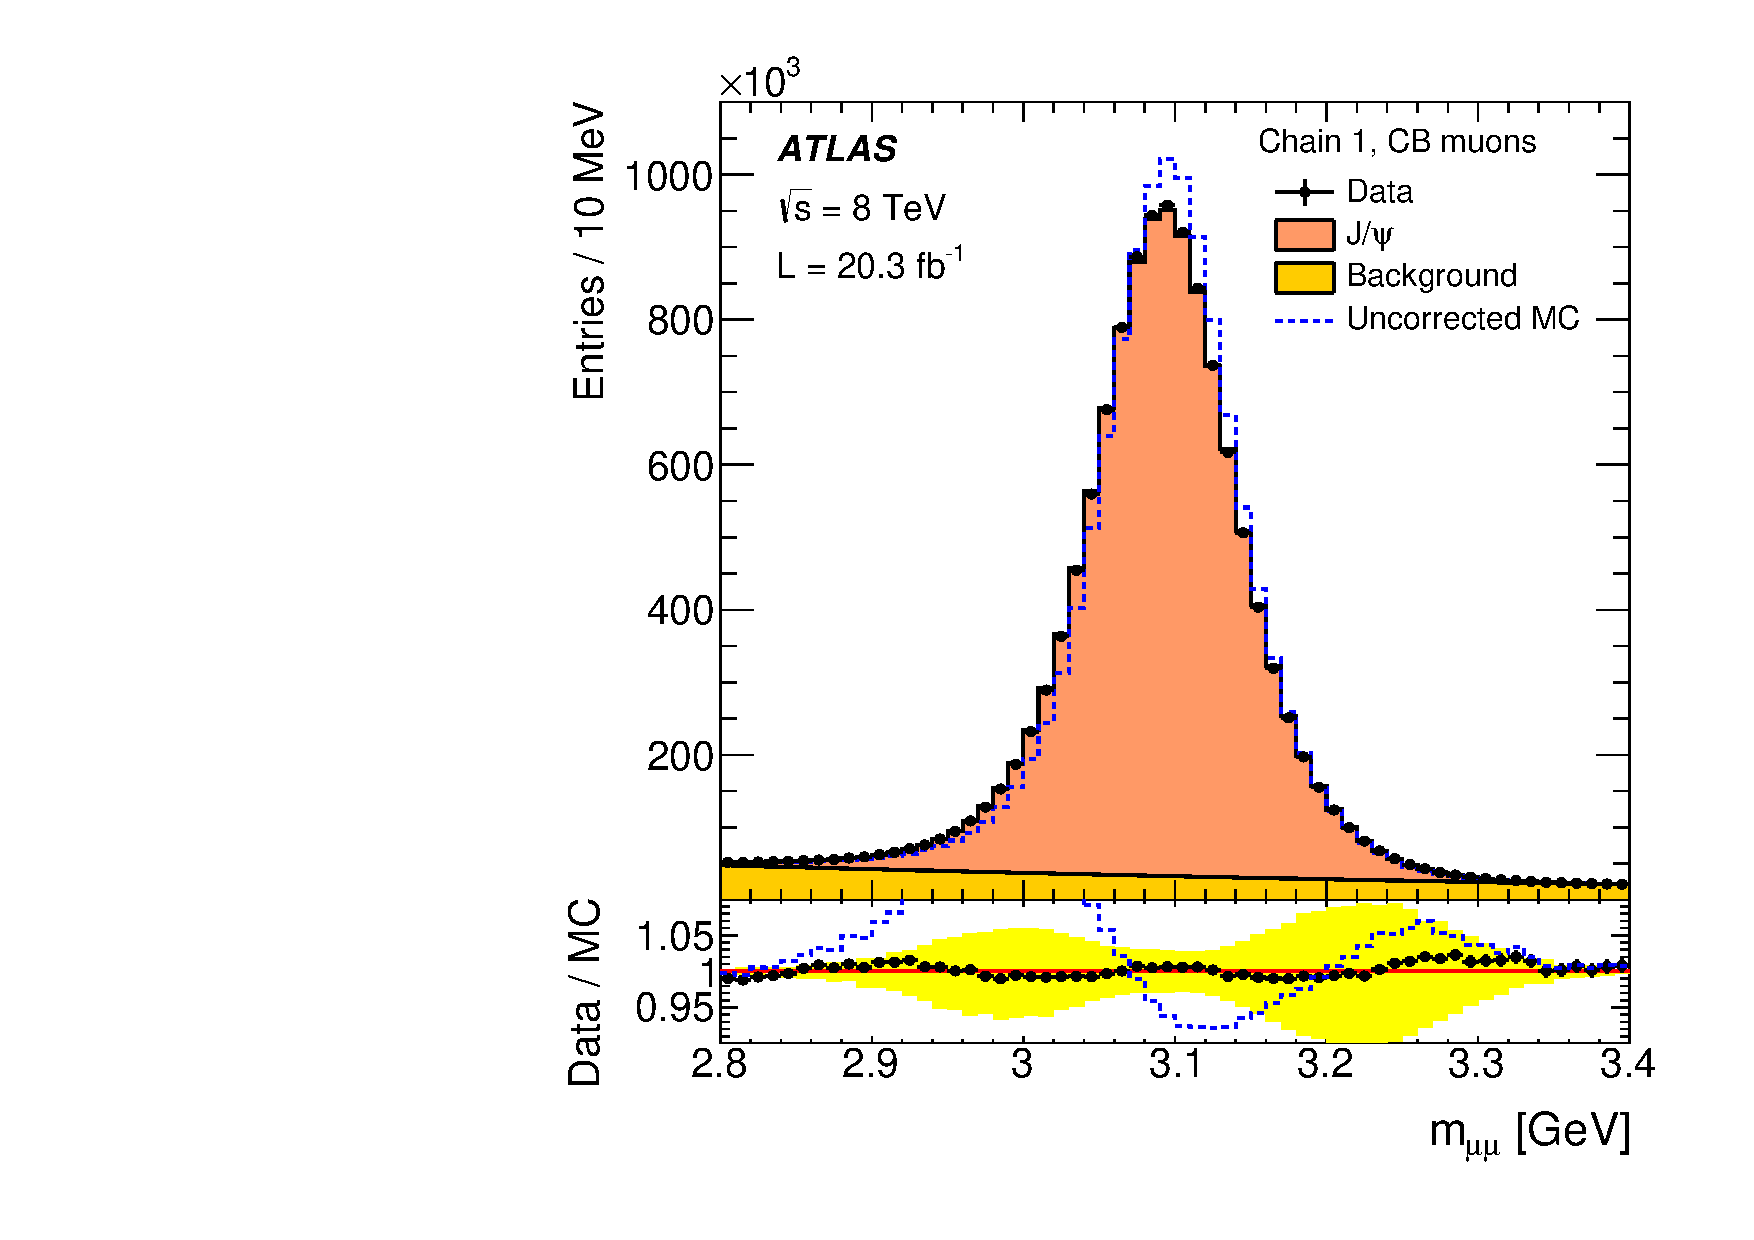
\includegraphics[width=\textwidth]{figures/STACO_jpsi_cb12.pdf}
	\caption{Run I. Taken from Ref~\cite{Aad:2014rra}}
\end{subfigure} % 
\begin{subfigure}{0.5\textwidth}
   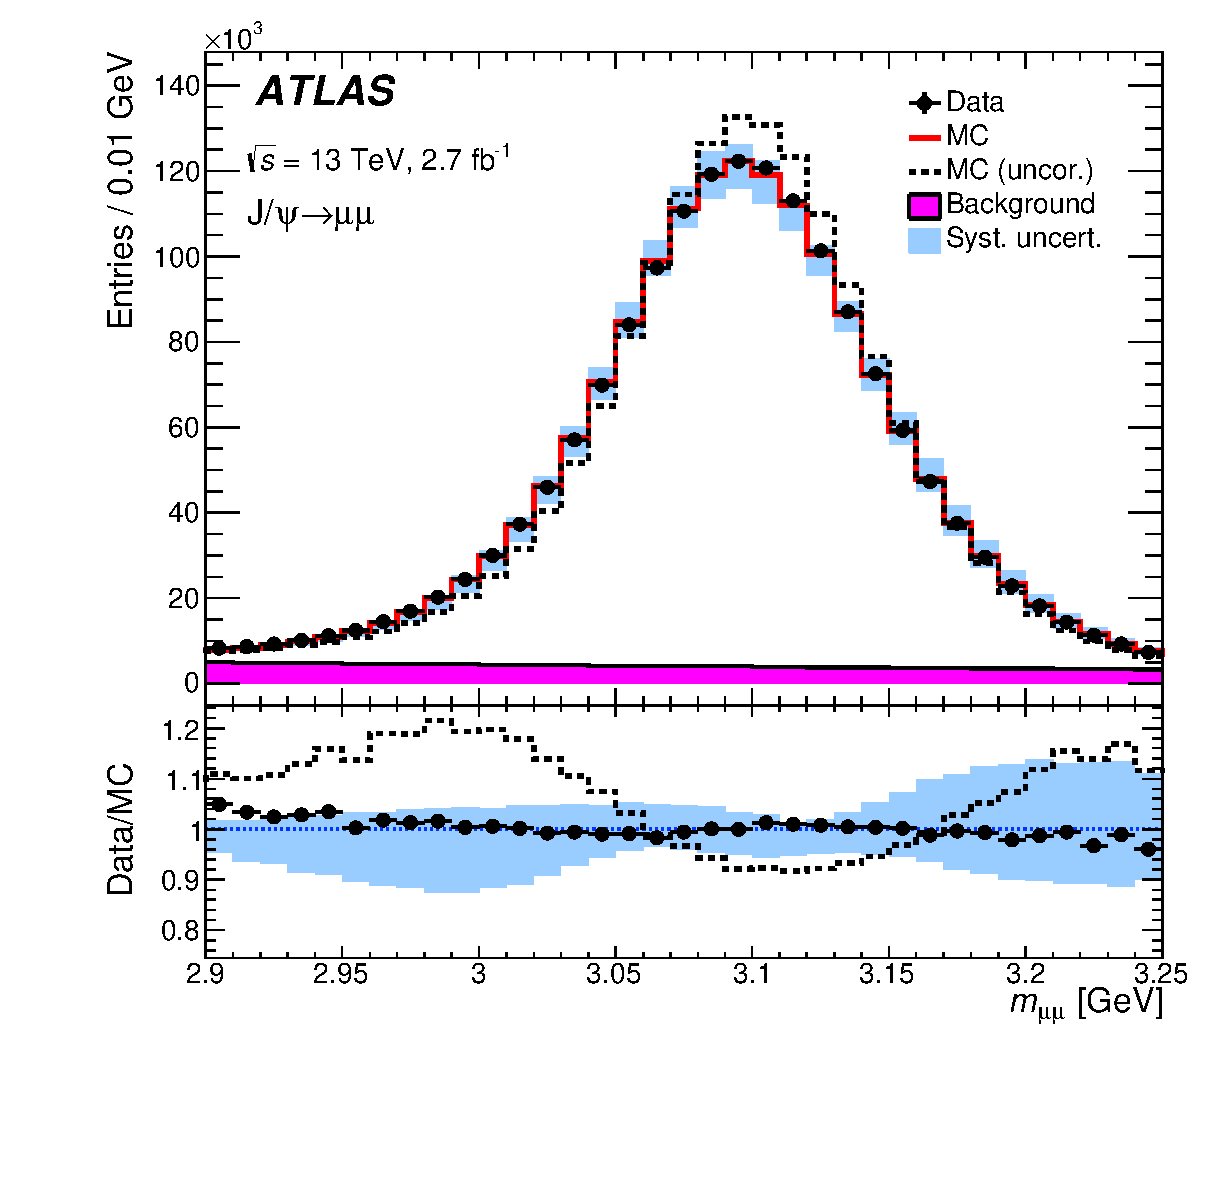
\includegraphics[width=\textwidth]{figures/fig_09_2.eps}
	\caption{Run II. Taken from Ref~\cite{Aad:2016jkr}}
\end{subfigure}
	\caption{Plots showing comparisons of $m_{\mu\mu}$ distributions for muons from \Jmm\ events in data, MC in 
which muon \pT\ is corrected and MC in which \pT is not corrected}
\label{fig:muScale}
\end{figure}

\par Systematic uncertainties in these corrections originate from imperfections in the model 
used for momentum correction, and in the fit used to extract correctional parameters. 
These were evaluated by varying several components when extracting the corrections. For example, the 
$m_{\mu\mu}$ window was varied by $\pm 5~\GeV$ in \Zmm\ event selection. This variation had the most impact 
effect on results.   
